\section{Positionierungs Algorithmen}
\label{sec:algorithmen}

\begin{frame}
  \frametitle{Algorithmen - Warum nicht GPS?}

  \begin{itemize}
  \item Vorteile
    \begin{itemize}
    \item sehr genau (1 bis 3 Meter)
    \item globale Position
    \item einfach zu Implementieren
    \end{itemize}
  ~\\
  \item Probleme
    \begin{itemize}
    \item schlechter Empfang in Gebäuden
    \item hohe Kosten
    \item zu groß und schwer für einen Sensorknoten
    \item hoher Stromverbrauch
    \end{itemize}
  \end{itemize}
\end{frame}

\begin{frame}
  \frametitle{Algorithmen}

  \begin{center}
    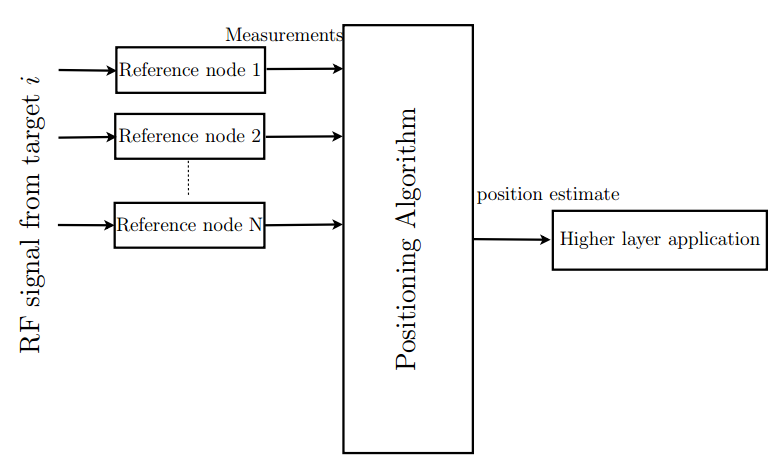
\includegraphics[scale=0.35]{img/algo_1}
  \end{center}
\end{frame}

\begin{frame}
  \frametitle{Algorithmen\footnote{Gholami, M. R. (2011). Positioning Algorithms for
      WirelessSensor Networks. Chalmers University of Technology.}}

  \begin{itemize}
  \item klassische Methoden
    \begin{itemize}
    \item Maximum-Likelihood
    \item Nonlinear least squares
    \item Linear least squares
    \end{itemize}
  ~\\
  \item Convex relaxation techniques
    \begin{itemize}
    \item Semidefinite Optimierung
    \item Second-order cone programming (SOCP)
    \end{itemize}
  ~\\
  \item Ansätze unter Verwendung der Mengenlehre
  \end{itemize}
\end{frame}
